\chapter{Optimization Algorithm}
\label{chapter:optimization}

An optimization problem is any problem where a function $f:X \rightarrow Y$ is given, and we search for the point $x \in X$ such that $f(x)$ is minimal or maximal. Obviously the minimum or maximum must not exist, as the example $f: (0, 1) \rightarrow \mathbb{R}, x \mapsto x$ demonstrates by not having either. Investigating conditions on $X$, $Y$ and $f$ such that a minimum or maximum exists is mathematically interesting. However, when implementing an optimization algorithm the true minimum or maximum can sometimes not be found even if it exists and is instead replaced by a sufficiently good approximation.

First we want to first think about some variations of the problem.

If a problem is stated to have additional conditions $P$ the minimum or maximum must satisfy we can consider the subset $M:= \{x \in X: P(x)\} \subseteq X$. By finding the minimum or maximum of $f: M \rightarrow Y$ a solution of the problem is solved. Once again such a minimum or maximum must not exist, even if we have that one is present in $X$.


In the example dealt with in this work we are given some data points $((x_k, y_k))_{k \in \{1, 2, ..., n\}}$ and want to find a close approximation in the form of a function $g(x, a_1, a_2, ..., a_m)$ where for every $a = (a_1, ..., a_m)$ we have a function $g_a(x) : \mathbb{R} \rightarrow \mathbb{R}, x \mapsto g(x, a_1, ..., a_m)$. Searching for a good approximation can be reformulated as searching for the minimum of $r(a) := \sum_{k=1}^{n} |g_a(x_k) - b_k|^2$ or any other error function. This form of optimization problem is called the Least Square Problem.

\subsection{Gradient Descent}

An iterative algorithm for finding the minimum of a differentiable function $f: \mathbb{R}^n \rightarrow \mathbb{R}$ is gradient descent. As the name suggests it uses information of the gradient $\nabla f$. Locally the negative gradient always points into the direction of greatest descent. The idea is to follow this direction for the next guess of the minimum. The pseudocode of this approach is given below.

\begin{algorithm}[H] \label{alg:gradient_descent}
	\SetAlgoLined
	\DontPrintSemicolon
	\LinesNumbered
	\SetKwInOut{Input}{input}
	\SetKwInOut{Output}{output}
	\caption{Gradient Descent}
	
	\Input{$f: \mathbb{R}^n \rightarrow \mathbb{R}$ ... differentiable, $x_0 \in \mathbb{R}^n$}
	\Output{$x \in \mathbb{R}^n$}
	\BlankLine
	\Begin{
		\For{$n=0$ \KwTo max\_iterations}{
			\If{improvement is smaller than threshold}{
				break\;
			}
			set or calculate step size $\gamma_n$\;
			$x_{n+1} = x_n - \gamma_n \nabla f(x_n)$\;
		}
		$x = x_n$\;
	}
\end{algorithm}

If we consider a function with a local but not global minimum gradient descent might not converge to the optimum. An example of such a function can be seen in figure~\ref{fig:grad_descent_global_min_not_found} along with the first values $x_n$ of gradient descent for a starting value not converging to the global minimum.

\begin{figure}[h]
	\centering
	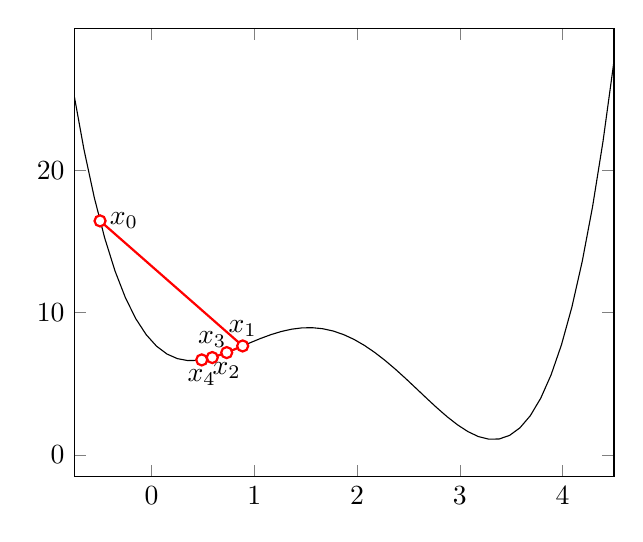
\begin{tikzpicture}
		\begin{axis}[xmin=-0.75, xmax=4.5, samples=100]
			\addplot[black] (x,x*x*x*x - 7*x*x*x + 14*x*x - 8*x + 8);
			\addplot[color=red,solid,thick,mark=*, mark options={fill=white}] 
			coordinates {
				(-0.5, 16.4375)
				(0.8875, 7.65428)
				(0.73223, 7.18773)
				(0.591558, 6.84009)
				(0.4894125, 6.67483)
			}; 
			\node [right] at (axis cs:  -0.5,  16.4375) {$x_0$};
			\node [above] at (axis cs:  0.8875, 7.65428) {$x_1$};
			\node [below] at (axis cs:  0.73223, 7.18773) {$x_2$};
			\node [above] at (axis cs:  0.591558, 6.84009) {$x_3$};
			\node [below] at (axis cs:  0.4894125, 6.67483) {$x_4$};
		\end{axis}
	\end{tikzpicture}
	\caption{The function has two local minimums. For this starting value and step size gradient descent approaches the local, but not global minimum.}
	\label{fig:grad_descent_global_min_not_found}
\end{figure}

Improvements can be made by choosing good step sizes, starting value or by starting with different values and comparing the results.

\section{Least Square Problem Algorithms}

% https://docs.scipy.org/doc/scipy/reference/generated/scipy.optimize.least_squares.html

We now focus on the Least Square Problem and give an introduction into various algorithms used.

Formally we are given a residual function $r_f(x)$ which tells us whether a function $f$ is a good approximation at the point $x$. We therefore want to find a way to minimize $||r(x)||^2$.

\subsection{Gauss–Newton Algorithm}

The idea behind this algorithm is that it is easy to find the intersection with zero of a linear function. If we linearize $r(x)$ locally we can approximate the root by finding it of the linear approximating function. This is demonstrated in figure~\ref{fig:approx_root_with_lin}.

\begin{figure}[h]
	\centering
	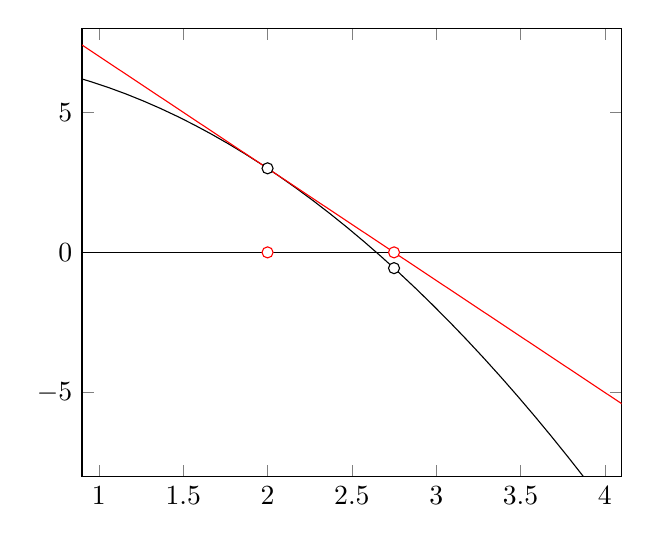
\begin{tikzpicture}
		\begin{axis}[xmin=0.9, xmax=4.1, ymin=-8, ymax=8, samples=100]
			\addplot[black] (x,-x*x + 7);
			\addplot[red] (x,-4*x+11);
			\addplot[black] (x,0);
			\addplot[color=black,only marks,mark=*, mark options={fill=white}] 
			coordinates {
				(2, 3)
				(2.75, -0.5625)
			};
			\addplot[color=red,only marks,mark=*, mark options={fill=white}] 
			coordinates {
				(2, 0)
				(2.75, 0)
			};
		\end{axis}
	\end{tikzpicture}
	\caption{By approximating the black function by a line an approximation of the root has been found.}
	\label{fig:approx_root_with_lin}
\end{figure}

Iterating this step of linear approximating gives us the Gauss-Newton Method. In figure~\ref{fig:gauss_newton_example} we can see that indeed $x_n$ seems to converge towards the root of the function.

\begin{figure}[h]
	\centering
	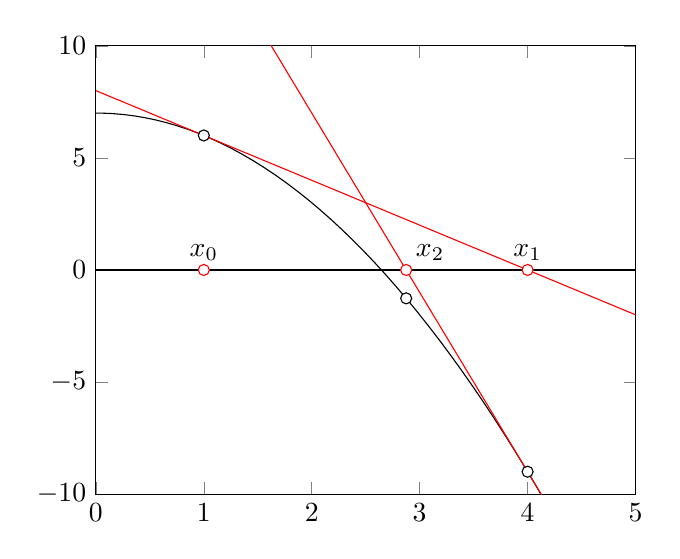
\begin{tikzpicture}
		\begin{axis}[xmin=0, xmax=5, ymin=-10, ymax=10, samples=100]
			\addplot[black] (x,-x*x + 7);
			\addplot[red] (x,-2*x+8);
			\addplot[red] (x,-8*x+23);
			\addplot[black] (x,0);
			\addplot[color=black,only marks,mark=*, mark options={fill=white}] 
			coordinates {
				(1, 6)
				(4, -9)
				(2.875, -1.265625)
			};
			\addplot[color=red,only marks,mark=*, mark options={fill=white}] 
			coordinates {
				(1, 0)
				(4, 0)
				(2.875, 0)
			};
			\node [above] at (axis cs:  1,   0) {$x_0$};
			\node [above] at (axis cs:  4,   0) {$x_1$};
			\node [above right] at (axis cs:  2.875,0) {$x_2$};
		\end{axis}
	\end{tikzpicture}
	\caption{Iteratively applying linear approximation gives the Gauss-Newton Method for approximating the root.}
	\label{fig:gauss_newton_example}
\end{figure}

Define $Dr$ as the Jacobian matrix $\left(\frac{\partial r_i}{\partial x_j}\right)_{ij}$. Using Taylor's theorem we get the linear approximation

\begin{align*}
	r(x) = r(a) + Dr(a)(x-a) + h(x)(x-a) \approx r(a) + Dr(a)(x-a) \text{ with } \lim\limits_{x\rightarrow a}h(x) = 0.
\end{align*}

Rewriting this as $r(x) \approx Ax - b$ where $A := Dr(a)$ and $b := Dr(a)a-r(a)$ gives us the algorithm for this method. As $Dr \in \mathbb{R}^{n\times m}$ we solve $Dr^T Dr x = Dr^T b$ in order to get a system with square matrix. If $n=m$ we can skip this step and get the so-called Newton algorithm as a variant.

\begin{algorithm}[H] \label{alg:gauss_newton}
	\SetAlgoLined
	\DontPrintSemicolon
	\LinesNumbered
	\SetKwInOut{Input}{input}
	\SetKwInOut{Output}{output}
	\caption{Gauss-Newton}
	
	\Input{$r: \mathbb{R}^n \rightarrow \mathbb{R}^m$ ... differentiable, $x_0 \in \mathbb{R}^n$}
	\Output{$x \in \mathbb{R}^n$}
	\BlankLine
	\Begin{
		\For{$n=0$ \KwTo max\_iterations}{
			\If{$x_n$ close enough to zero}{
				break\;
			}
			Calculate $A_n := Dr(x_n)$\;
			Calculate $b_n := A_n x_n - r(x_n)$\;
			Solve $A_n^T A_n x_{n+1} = A_n^T b_n$\;
		}
		$x = x_n$\;
	}
\end{algorithm}

Gauss-Newton is guaranteed to find a local minimum $x$ if $r$ is twice continuously differentiable in an open convex set including $x$, $Dr$ has a full rank and the initial value is close enough to $x$.

For the example demonstrated in figure~\ref{fig:gauss_newton_fails_sin} we can see that choosing a particular starting value leads to a loop in which only two points are explored as possible roots. More extreme examples exists in which Gauss-Newton gets increasingly further away from the root, due to an increasingly flat incline the further we get from the root. One example of such a function can be seen in figure~\ref{fig:gauss_newton_fails_cubic_root}.

\begin{figure}[h]
	\centering
	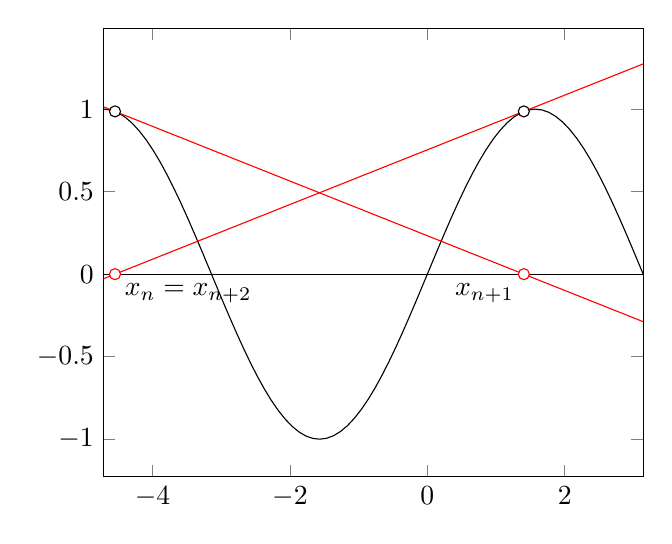
\begin{tikzpicture}
		\begin{axis}[xmin=-4.71238898, xmax=3.141592653, samples=100]
			\addplot[black] {sin(deg(x))}; 
			\addplot[red] (x,-0.165738017518283266*x+0.23274423977441288);
			\addplot[red] (x,0.16573801751814743279*x+0.75342557803057879409);
			\addplot[black] (x,0);
			\addplot[color=black,only marks,mark=*, mark options={fill=white}] 
			coordinates {
				(-4.54588264848318, 0.9861698178047780981)
				(1.4042899948935245, 0.986169817804800926611)
			};
			\addplot[color=red,only marks,mark=*, mark options={fill=white}] 
			coordinates {
				(-4.54588264848318, 0)
				(1.4042899948935245, 0)
			};
			\node [below right] at (axis cs:  -4.54588264848318, 0) {$x_n=x_{n+2}$};
			\node [below left] at (axis cs:  1.4042899948935245, 0) {$x_{n+1}$};
		\end{axis}
	\end{tikzpicture}
	\caption{For a poor choice of starting values Gauss-Newton can never find the root of the function $\sin(x)$.}
	\label{fig:gauss_newton_fails_sin}
\end{figure}

\begin{figure}[h]
	\centering
	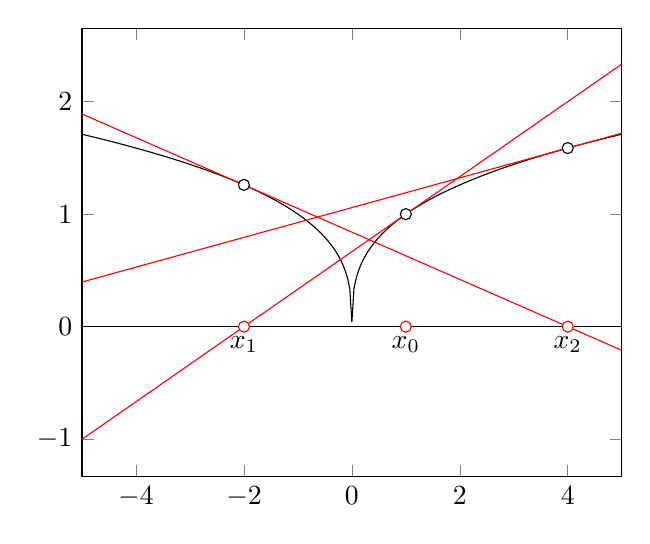
\begin{tikzpicture}
		\begin{axis}[xmin=-5, xmax=5, samples=257]
			\addplot[black] {abs(x)^(1/3)};
			\addplot[red] (x,0.33333333*x+0.666667);
			\addplot[red] (x,-0.209987*x+0.839947);
			\addplot[red] (x,0.132283*x+1.05827);
			\addplot[black] (x,0);
			\addplot[color=black,only marks,mark=*, mark options={fill=white}] 
			coordinates {
				(1, 1)
				(-2, 1.25992)
				(4, 1.5874)
			};
			\addplot[color=red,only marks,mark=*, mark options={fill=white}] 
			coordinates {
				(1, 0)
				(-2, 0)
				(4,  0)
			};
			\node [below] at (axis cs:  1, 0) {$x_0$};
			\node [below] at (axis cs:  -2, 0) {$x_1$};
			\node [below] at (axis cs:  4, 0) {$x_2$};
		\end{axis}
	\end{tikzpicture}
	\caption{Finding the root of the function $\sqrt[3]{|x|}$ using Gauss-Newton is only possible if the starting value $x_0$ is chosen as $0$, which is the root. For any other value we have that the guess gets further and further away. Indeed for any $x_n$ we have $x_{n+1} = -2x_n$.}
	\label{fig:gauss_newton_fails_cubic_root}
\end{figure}

Both problems, the starting value being too far from the root and the $Dr$ not having full rank, can be combated using the technique of dampening. Instead of moving the new guess all the way to the root of the linear approximation we only move part of the way. How much can be determined by a dampening factor $\lambda_n$ or a constant $\lambda$.

\subsection{Levenberg-Marquardt Algorithm}

\subsection{Trust Region Reflective Algorithm}
% https://www.applied-mathematics.net/LMvsTR/LMvsTR.pdf

% https://johnwlambert.github.io/gauss-newton/

\subsection{Dogleg Algorithm with Rectangular Trust Regions}